% -----------------------------------------------
% Template for SMC 2009
%     smc2009.sty -> style file
% Last modified by Fabien Gouyon (smc2009@inescporto.pt)
% Modified by Juan P. Bello (ismir2008-papers@ismir.net)
% By Rainer Typke (ismir07.rainer@safersignup.com)
% Based on the 2004 template by Eloi Batlle.
% -----------------------------------------------

\documentclass{article}
\usepackage{smc2009,amsmath}
% To use when using pdflatex
\usepackage{graphicx}
\usepackage{url}     
\usepackage{hyperref}   
      
\newenvironment{packed_item}{
\begin{itemize}
  \setlength{\itemsep}{1pt}
  \setlength{\parskip}{0pt}
  \setlength{\parsep}{0pt}
}{\end{itemize}}

\newenvironment{packed_enumerate}{
\begin{enumerate}
  \setlength{\itemsep}{1pt}
  \setlength{\parskip}{0pt}
  \setlength{\parsep}{0pt}
}{\end{enumerate}}
% To use when using latex, dvips and ps2pdf
% \usepackage[dvips]{graphicx}

% Title.
% ------
%\title{a layered approach to sound spatialization - concepts and examples}
\title{A stratified approach for sound spatialization}
% IMPORTANT NOTICE:
% Reviews are double-blind
% Authors will not be informed of who reviews their papers, and author names will be concealed from the reviewers 
% Please avoid evident self references in the text

% Authors' names must be omitted from title page (or listed as �name(s) omitted for submission�)


% Single address
% To use with only one author or several with the same address
% ---------------
%\oneauthor
%   {Author} {School \\ Email}

% Two addresses
 %--------------
\twoauthors
  {First author} {School \\ Email}
  {Second author} {Company \\ Email}

% Three addresses
% --------------
%\threeauthors
%  {First author} {School \\ Email}
%  {Second author} {Company \\ Email}
%  {Third author} {Company \\ Email}


\begin{document}
%    
\sloppy
\maketitle
%

\permission

\begin{abstract}
The improvements in computer and audio equipment in recent years makes it possible to experiment more freely with resource-demanding sound synthesis techniques such as spatialization. For seeking new means of expression different spatialization applications should be easily combined and accessible for both programmatic and user interfaces. % and/or other controllers. %e.g. a generative mapping of a granular synth output to different spatial renderer from one common user interface, while also streaming spatial encoded audio to the internet. 
Guaranteeing efficient workflow for non-standardized approaches requires structure, flexibility, and interoperability. Common spatialization systems are too often self-contained giving no consideration to these requirements. Therefore, we propose a multi-layer approach to mediate sound spatialization to meet these demands.\\                              	
\textbf{Keywords:} sound spatialization, interoperability, layered architecture, adaptation, site-specific, Ambisonics , TODO: make better \& stronger keywords   
%-flexible working environment for spatialization\\
%-A layered approach towards interoperability in sound spatialization management\\
%The abstract should be placed at the top left column and should contain
%about 150-200 words.
%stratified     strata  stratum 
%KEYWORDS : 
\end{abstract}

\section{Introduction}\label{sec:introduction}       
The goal of any spatialization
%rendering is it only the rendering system, or control/rendering ?
system is to facilitate or empower the creative use of the spatial medium for a sonic artist. Quantitative studies on spatial music (\cite{otondo2008ctu}, \cite{PetersSurvey}) remind us that there are great individual and context-related differences in defining that goal amongst artists. %that the compositional use of spatialization techniques varies strongly across composers and musical context.    
The requirements of a computer aided spatialization system may vary between a fixed-media composition (e.g \cite{BarrettOS02}%TODO: find a Robert Normandeau reference
), an art-installation (\cite{lossius:2007sound_space_body}), and a live diffusion performance (\cite{Truax99}). 
One example is an interactive art installation where the real-time quality of a spatial rendering system is of great importance in combination with the possibility to control spatial processes through a multi-touch screen.  Juxtaposed is a second example: a performance of a fixed-media composition where the paramount features may be multichannel playback and the compensation of non-equidistant loudspeakers (in terms of sound pressure and time delays). Additional scenarios may require binaural rendering for headphone listening, multichannel recording, up and down mixing, or a visual representation of a sound scene.  
Moreover, even during the creation of one spatial art work, the importance of these requirements may change throughout different stages of the creative processes. % \emph{Experimentation -- Arranging -- Performance -- Documentation}. 
%Several common paradigms for spatial sound synthesis are outlined in section \ref{sec:review}. %The availability of better CPU resources in recent years makes it possible to experiment more freely with these paradigms for seeking new ways of expressions, e.g. a generative mapping of a granular synth output to different spatial renderer from one common user interface, while also streaming spatial encoded audio to the internet. This paper shows how such complex spatialization scenarios can be conceptualized through a multi-layer structure.    



%\begin{packed_item} 
%	\item {real-time or non real-time rendering}  
%%	\item {Plug-In structure: exchangeable renderer and interface components} - this is one of the ideas of the article, we don't need it here
%	\item {multichannel playback and recording possibility} 	
%	\item {binaural rendering for headphone listening}
%	\item {testing technical setup, e.g. loudspeaker connections}   
%	\item {customizable renderer in order to accommodate for different acoustical conditions, e.g. adapting the virtual room description to the listening room} 
%\item {customizable to accommodate for different technical conditions, e.g. rendering to different reproduction formats, compensation for non-ideal loudspeaker configurations, routing signals to dedicated physical outputs}  
%	\item {visual representation of a sound scene} 
%\item {separate render and control layer} - this is one of the ideas of the article, we don't need it here
%\item {allowing for external control e.g. through MIDI, OSC or other protocols}
%
%\end{packed_item}
%TODO: this list must become better!-please help - \emph{what do we want to say with this list ??} \\

%The outlined requirements may differ according to artistic paradigms.
%-Use cases (users : composers, installation artists, scientists...etc...)
%   - OpenMusic off-line rendering
%   - BEAST sound diffusion (the more speaker - the mre complicated to perform)
%   - interactive sound installations
%   - real-time control via sensors/gestural controller etc. by performer
%   - tape-music (fixed media)
%   - computer generated - real time spatialization (see <meta-description> layer)
   
    
%Experimental stage:\\
%\begin{packed_item}
% \item {Plug-In structure: exchangeable renderer and interface components} 
% \item {multichannel recording possibility for capturing of sketches/ideas}         
% \item {present management}
% \item {sound scene visualization - especially for off-line rendering of spatial processes}
%\end{packed_item} 

%Compositional stage:\\  
%\begin{packed_item}
%  \item {binaural rendering for headphone listening} 
%\end{packed_item} 
%Performance stage:\\
%\begin{packed_item} 
%	\item {customizable to accommodate for different technical conditions, e.g. rendering to different reproduction formats, compensation for non-ideal %loudspeaker configurations, routing signals to dedicated physical outputs}   
%    \item {testing technical setup, e.g. loudspeaker connections}
%    \item {customizable to accommodate for different acoustical conditions, e.g. adapting the virtual room description to the listening room} 
%\end{packed_item} 
%Documentation stage:\\  
%\begin{packed_item}
%\item {multichannel recording possibility}         
%\item {storing }       
%\end{packed_item}  


%\quote{ What WE need, for our personal work, is a way to extend the capabilities of those tools in a completely flexible and configurable way - and that suggests plug-ins (though it will always be a potential problem overcoming inherent IO structures in the host applications).}

%\quote{working with non-standard loudspeakers: Meyer Sound Spherical Loudspeaker Array that is under research at CNMAT, or the Hemisphere Point-source Emanation Loudspeaker, for example.  I would like to experiment with these;}

%\quote{Tool building and music making happen together and depend upon each other.}

%\quote{Very frustrated with my current spatialization software and am desperately looking for something better!}

\section{Review of current Paradigms} \label{sec:review}
%This section gives an overview of current paradigms and solutions for sound spatialization, and shows their limitations. 
\subsection{Live sound diffusion}  
?? shall we mention live diffusion as a paradigm ?
\subsection{Digital Audio Workstations - DAW} \label{sec:digital audio workstations - DAW} 
Currently, many composers and sound-artists use DAWs for designing their sound spatialization primarily in the context of fixed media, tape-music, and consumer media production. Users of DAWs often have former experience with live diffusion systems, or with panning in a hardware mixing console. Their migration to DAWs seems reasonable because the linear time representation of sound material and the audio bus architecture in DAWs originates from the use of multitrack tape recorder and mixing consoles. 
A number of (mainly commercial) DAWs are mature and offer a systematic user interface, good project and sound file management, and extendability through plug-ins.  They can fulfill the needs of many users in the described context.\\
However, through focusing on consumer media products, multichannel capabilities are limited. ITU 5.1, a surround sound format with equidistant loudspeakers around an ideal located listener and originally designed for the requirements of the film industry, is the most common multichannel format in DAWs and in surround panning plugins. 
Moreover, the 5.1 setup favors frontal direction and has limited capabilities for localizing virtual sources from the sides and back, which may limit its artistic use.  More recently, extensions to 7.1 or 10.2 are available\footnote{A comparison of DAWs concerning their multichannel audio capabilities shows \url{http://acousmodules.free.fr/hosts.htm}.}.   
Non-commercial loudspeaker setups are used in art installations or concert hall environments varying in number and layout.  These configurations are not typically anticipated by existing DAW software. Consequently, existing DAW-projects are difficult to adapt to these situations. 
%From 1993, emergence of the ITU 5.1 has been announced as a major improvement for mixing surround sound. Originally designed to fulfill the needs of the film industry, this loudspeaker configuration appeared to music and entertainment companies as a new way to extend their commercial offer. Since then, all DAWs surround panners have been designed to respect and organize sound processing for this set-up. It was not until the late nineties that new suggestions for surround workstations (from 6.1 to 10.2, enhancing sides precision, and perception outside of the Central Listening Position) were considered.\\
%This was an useful approach for recording, multimedia or film prospects (cannot do business without standards), but still in a regular, circular, geometric and (FIXME: non-neutral ?we mean it influences the user) design, which cannot be acceptable and sufficient for creation or live applications. As an example, a non-flexible loudspeaker circle set-up is very rarely adapted to the concert hall.\\ 
\\Another critical function for surround sound mixing is the means by which a sound source's energy is distributed amongst the loudspeakers. A \emph{blur} parameter, which determines the apparent source width of a panned signal, should be a standard control element of every surround panner because it enables many variations and possibilities for a creative mix. %and because we would work with this parameter considering the specific features of the sound we have to spatialize. 
In most applications, this factor is restricted and linked to the sound source's position relative to the center in the surround panner, and is related to parameters such as \emph{spread} or \emph{diversity} (e.g. in Apple Logic Pro \footnote{\url{www.apple.com/logicstudio/}}). To the authors' opinion, the most flexible control element can be found in Sequoia \footnote{\url{http://www.magix.com/us/sequoia/}}, with \emph{soundfield} offset and character (shape) settings for each track, a \emph{global divergence} to fit to the listening room size, and a complete flexibility for the speaker set-up in the listening area. 
%
%
% Did we discuss all point below:? (moved above -> we should use them at the beginning IMHO)
%
%
%spatialization is mainly done in DAWs and leads to "panning" because the bus architectures and interfaces of the panning plugins suggests this.
%    Limitations:
%        a) mainly tied to consumer formats (stereo and ITU 5:1 surround)
%        b) restricted to linear prerendering compositional processes
%        c) complicated to maintain automation when changing rendering plugIn
%        d) burden to connect interfaces (Lemur, Stantum, Wacom, Camera-tracking)
%        
% 
      
\subsection{Media programming environments}  \label{sec:Media programming environments}
Beside the paradigm of the DAW, various media programming environments exist that are capable of spatial sound synthesis. These include SuperCollider, Pure Data, Chuck, OpenMusic, and Max/MSP.  In order to support individual approaches and to meet the specific needs of computer music and mixed media art, these environments enable the user to combine music making with computer programming.\\  
However, in the name of complete flexibility, these environments lack in providing structured solutions for the specific challenges of spatial music as outlined in section \ref{sec:introduction}. Consequently, numerous self-contained spatialization libraries and toolboxes have been created by artists and researchers to generate virtual sound sources and artificial spaces.  These include the Space Unit Generator \cite{SUG02}, IRCAM's Spatialisateur \cite{JotPhD}, and Virtual Microphone Control \cite{CMJ08-VIMIC}. Also toolboxes primarily dedicated to sound diffusion practice, such as the BEASTmulch System\footnote{\url{http://www.beast.bham.ac.uk/research}}, or ICAST \cite{ICAST06} are available.   
Each tool, however, may only provide solutions for a subset of compositional viewpoints.  The development of new aesthetics through combining these tools is difficult or limited through their specific designs. 

\section{Strategies \& Methodologies in sound spatialization}  
 
A traditional workflow in electroacoustic composition or linear sound editing comprises a number of steps leading to the construction of the audio scene. Other contexts such as audio installations or interactive/multimedia work imply a different sequence in the steps of the process. The modular approach tries to abstract these differences and define underlying common elements that are always in play when spatialization is used. This layer model doesn't imply a specific method, it much rather tries to emphasize the importance of the interchangeability of modules, which share their interconnecting interfaces. The tools for each layer can be exchanged and compared, without forcing the artist to completely rebuild their setup.

\begin{quote}Spatial orchestration eases this [...] constraint, [...] the composition may be reconfigured for each individual performance. This will require [...] the composer [to] conceive spatial attributes in a more abstract fashion, that is then instantiated in potentially different ways into different performance environments. \cite{Lyon:2008spatial_orchestration} \end{quote}
By working symbolically during the composition/editing process and separating the authoring from the rendering processes a realization can become portable. A common set of descriptors and shared representation metaphors such as timelines or scene graphs builds the glue to make a disparate set of tools into a coherent workflow by enhancing interoperability between the different building blocks.\\
Modularity is another essential tenet.  Modularity allows the separation of elements into different layers according to their function as described in \ref{sec:layers}.  Furthermore, Modularity provides a means by which   modules may query additional modules and then adapt themselves to other parts of the graph.\\
The Tools used for authoring or rendering must comply to these recommendations, and can be separated in two categories : rendering engines and authoring meta-tools.\\


\subsection{A layered approach to the spatialization workflow}\label{sec:layers}
%TROND, J45CH\\
In order to better grasp the structural and methodological entities used in a spatialization process, a layered approach is proposed, which defines the problem domains in an ascending order of abstraction (Table \ref{fig:layers}). This model gets its inspiration from the OSI network model \footnote{\url{http://en.wikipedia.org/wiki/OSI_model}}. OSI (Open Systems Interconnection), is an abstract description for layered communications and computer network protocol design, which divides network architecture into seven layers which range, from top to bottom, between the Application and the Physical Layers
%
%
%\begin{packed_enumerate}   
%\item[5.]{controlling the rendering (e.g. HoloEdit, ambicontrol, swarms, boids \cite{kimboyle:ssp}, trajectories...)     <indirect control %description or meta-description>
%       Protocol: SpatDIF extended }
%\item[4.]{position of sources and speakers at one moment in time as SpatDIF                          <direct control description>
%       Protocol: SpatDIF core, SpatDIF extended if required by the encoder }
%\item[3.]{encoded audio
%       Protocols:
%           Spatial infomation embedded in format: (e.g. B-format and Dirac, MPEG-surround ?)
%           SpatDIF core and extended if required by the encoder (concerning info on target system) }
%\item[2.]{decoded audio
%       Protocols: E.g. CoreAudio, Jack, PortAudio }
%\item[1.]{physical layer (computers, sound cards, speakers, etc.)}
%\end{packed_enumerate}  
%TODO: sketch of the layers?
%
%\begin{table*}   
%	\begin{tabular}{llll} 
%	Nr. & Layer & Examples&\\
%	\hline
%	5. & controlling the rendering & Holo-Edit, ambicontrol,& indirect control description \\ 
%	  &    &  swarm simulator, algorithmic generator & or meta-description\\       %, boids \cite{kimboyle:ssp}
%	\hline
%	4. & audio scene description  & Protocol: SpatDIF core protocol,  & current position of virtual sound sources, \\
%	   &             &    SpatDIF extended if required  & loudspeakers, source width, ...\\
%	\hline
%	3. & encoded audio Protocols & B-format, DIRAC, MPEG-surround & Spatial information embedded in format\\
% 	\hline 
%	2. & decoded audio Protocols & CoreAudio, Jack, PortAudio & \\	
%	\hline
%	1. & physical layer & computers, sound cards, loudspeakers& \\			 
%	%\hline
%	%Distinctness & ??& ??\\			
%   	\end{tabular}               
%  			\caption{Layers}
%		\label{tab:layer}       
%	\end{table*}                          
	\begin{figure}
		[ht] \centerline{
		\includegraphics[width=1.1\columnwidth]{layers.pdf}} \caption{TODO: where is Soundflower and Rewire in that graph?} \label{fig:layers} 
	\end{figure}
	%\end{center}  
\subsubsection{Physical Device Layer}
TODO 
\subsubsection{Decoded Audio Stream Layer}
TODO
\subsubsection{Encoded Audio Stream Layer}	
TODO
\subsubsection{DSP / Rendering Layer}
TODO
\subsubsection{Audio Scene Description Layer}
TODO \\
\textbf{SpatDIF:} A particular effort has been done by the authors on integrating and developing SpatDIF as Layer 4 (audio scene description). The goal of SpatDIF is to develop a system-independent language for describing spatial audio scenes \cite{Peters:2008spatdif} 
Formats that integrate spatial audio descriptors such as MPEG-4 Advanced Audio BIFS or OpenAL did not fully succeed in the music or fine arts community because these formats are primary tailored to multimedia and gaming applications and do not necessarily consider the special requirements of spatial music and performances in concert venues or sonic/mixed media installations in specific places such as galleries or museums. Furthermore it is the authors' opinion that artists were not sufficiently involved in the development of these formats.\\
As can be seen in the layer section (... to be continued ...)

\subsubsection{Authoring / Render-Control Layer}	
TODO   

\section{Stratified Tools}
%- structured according to layers
In order to concretely experiment these ideas, the authors designed and used the tools described below :
TODO: maybe the tools should be organized according to the layers 
\subsection{ICST Ambisonics}
The ICST ambisonics tools comprise a set of four externals for Max/MSP. The two DSP externals ambiencode~ and ambidecode~ generate and decode Higher Order Ambisonics. They reach 3rd order with Furse-Malham Formulas in version 1.2, and 5th order using either the Furse-Malham or Normalized 3D formulas in version 2.0. The two control externals ambimonitor and ambicontrol complete the set. Ambimonitor presents the user with a GUI displaying point sources in an abstract 2D or 3D space, various key commands, snapshot and file I/O capabilities and it generates coordinate information for the DSP objects. Ambicontrol provides a number of methods that control motion of points in the Ambimonitor's dataset. Automated motions such as rotation, random motion, optionally constrained in bounding volumes and user defined trajectories can be applied to single or grouped points. The import/export format for the trajectories and state snapshots is a simple XML text file, which will be replaced by a SpatDIF compliant formatting in a next release. \cite{Schacher:2006ambi_max} At ICST a different panning algorithm \cite{Neukom:2008ambipan} was derived from in-phase ambisonic decoding and also coded as Max/MSP external. Ambipanning~ implements the Ambisonic Equivalent Panning, which transcodes in one step a set of mono sources onto a ideally circular speaker setup with an arbitrary number of speakers. The algorithm works with a continuous order factor, which permits to apply per point individually varying directivity responses. This external understands the same command syntax and becomes interchangeable with the other ICST ambisonic DSP objects. 
\subsection{Jamoma}

Jamoma\footnote{\url{http://www.jamoma.org/}} is a collaborative set of software tools.  It includes DSP libraries and a framework for structuring Max/MSP patches.\\
The DBAP algorithm \cite{dbapICMC09} is included in the Jamoma library as a Max/MSP external. DBAP focuses on applications that extend beyond traditional loudspeaker arrangements.  Limitations explained in \ref{sec:digital audio workstations - DAW}, based on an ideal model rather than actual positions of loudspeakers in the room, can thus be overcome.  DBAP has proven to be particularly useful in theatre and installation applications.\\
In addition to the libraries, the Jamoma Modular Framework\cite{Place:2006jamoma} supplies a set of spatialization tools as modules wrapping various spatialization algorithms (VBAP \cite{Pulkki:2000vbap_max}, DBAP \cite{dbapICMC09}, ambisonics \cite{Schacher:2006ambi_max}, and ViMic\cite{CMJ08-VIMIC}) that can be combined and substituted with each other to quickly compare, audition, or adapt each of them to a specific context. 
Moreover, a number of effect processors (Doppler, Airfilter, RollOff, Reverb) and utilities (loudspeaker setup, FIXME:SPL compensation, FIXME:delay compensation, multichannel meters and auxiliaries) are also available in the distribution.
All these modules have been designed according to a common namespace model, thus allowing the user to seamlessly connect the modules in minutes and then experiment with the ideas presented here.  In particular, the  interoperability of different algorithms such as Holo-Edit, ICST Ambimonitor, and physical interfaces (i.e. JazzMutant's Lemur \footnote{\url{http://www.jazzmutant.com/}} or TUIO-compliant \cite{kaltenbrunner2005tpt} devices using the Max Multitouch Framework \footnote{\url{http://code.google.com/p/mmf/}}) can be quickly mapped to the aforementioned rendering models.\\
Current low-level spatial-systems research in Jamoma is focused on the development of Jamoma Multicore \footnote{\url{http://code.google.com/p/jamulticore/}}, a coding layer for the creation of dynamic audio graph topographies.  One application of Jamoma Multicore is the creation of ``multichannel signals" that can be passed between objects in Max/MSP or Pure Data.  These multichannel signals are also dynamic, meaning that the number of channels can be changed instantaneously and the audio graph will adapt accordingly.  The signals can be audio in the traditional sense, or carried ambisonics encoded signals of the Nth order.

 
\subsection{Holo-Edit}
Initiated by L. Pottier \cite{PottierDAFX98}, Holo-Edit is part of the GMEM Holophon project and dedicated to multi-sources and multi-speakers spatialization. This standalone application \cite{Pottier05} is written in Java / OpenGL and uses the timeline paradigm found in traditional DAW for recording, editing, and playback of spatialization control messages. The data is manipulated in the form of trajectories or sequences of time-tagged points in a 3D space. These trajectories can be generated or modified by an expandable set of tools allowing specific spatial and temporal behaviors, including symmetry, proportion, translation, acceleration, local exaggeration and more. Different scene representation windows allow the user to view and modify data focusing on different aspects: \emph{Room} by a top view of the virtual space, \emph{Time Editor} which is related to the classic automation curve view in DAWs and \emph{Score} which represent the whole composition in a multi-track block-based view.\\
An important feature of Holo-Edit is the ability to represent sound waveforms beside their trajectories. This allows to synchronize sound cues to their associated movements.
The model of space/time representation has been left intentionally generic, thus it can control a variety of different spatialization methods and auditory virtual environment such as \cite{CMJ08-VIMIC}. %Even if Holo-Edit is combined with a auditory virtual environment such as \cite{CMJ08-VIMIC}, its generic nature allows to use it in a more abstract way, thinking more of movements in an arbitrary space ( may it be acoustic, symbolic, semiotic ...).[TODO: I changed something here, but I don't know what you really mean] [ FIXED BY CHARLES : I wanted to point that the movements composed are not made to be strongly linked with the scales of our physical world. But we can absolutly erase this line as it's not fundamental, was just a note ]
Holo-Edit uses Open Sound Control (OSC) as a communication protocol. It has been successfully used in different media environments as mentioned in section \ref{sec:Media programming environments}  using various spatial renderers, such as VBAP, Ambisonics, or DBAP. 
In this scenarios, the main challenge is to adapt and format the data stream to fit the specific algorithm syntax (e.g. coordinate system, dimensions, units).
Consequently a communication interface has been developed and integrated into Jamoma as a first step towards SpatDIF compliancy of Holo-Edit. It thus adds the features of playing trajectory compositions with the associated sound cues according to the edited score and to record them from any real-time control inputs available in Jamoma. 
  


\section{Discussion \& Outlook}

TODO : Here we should maybe emphasize the fact that all these tools do work together and insert a screenshot of a patch demonstrating this (like the one I committed yesterday in UserLib/Holophon/Examples/LemurThingie) - and maybe a graph showing the connections... ???

The method used here tries to define standards through experimental implementation and usage :

This collaborative research has emerged from a workshop... we're planning to make more of them

The next step includes developing more use cases and a wider set of tools. SpatDIF and the modular approach to spatialization needs to grow through implementations in a variety of software, especially commercially used systems DAWs and plugins.


\section{Conclusion}
A conclusion is the place when you get tired of thinking. \\

\section{Acknowledgment}
\bibliographystyle{abbrv}  %\bibliographystyle{natbib}% ama, nar, alpha, plain, chicago,{plainnat}  abbrv, siam   
\small
\bibliography{smc09}
\end{document}   

%%%%%%%  Poubelle %%%%%%   
	
%\subsection{Frameworks for Spatialization}
%\textbf{Spatialisateur} (Spat) \cite{JotPhD}, in development at IRCAM and Espaces Nouveaux since 1991, is a library of spatialization algorithms for Max/MSP, including VBAP, first-order Ambisonics and stereo techniques (XY, MS, ORTF) for up to 8 loudspeakers. It can also reproduce 3D sound for headphones (binaural) or 2/4 loudspeakers (transaural). A room model is included to create artificial early reflections and reverb controlled by a perceptual-based user interface.\\
%\textbf{Ambisonics toolbox}  \cite{Schacher:2006ambi_max}

   

% \section{Style Stuff - delme}

% \subsection{Title and Authors}

%The title is 14pt Times, bold, caps, upper case, centered. Authors' names are centered. 
%The lead author's name is to be listed first (left-most), and the co-authors' names after. If the addresses for all 
%authors are the same, include the address only once, centered. If the authors have different addresses, 
%put the addresses, evenly spaced, under each authors' name.

% Reviews are double-blind. {\it \textbf{Author information should be removed from this page in initial submissions}}, 
% and only added later by the authors when sending camera-ready versions.


%\subsection{Figures, Tables and Captions}

%All artwork must be centered, neat, clean, and legible. All lines should
%be very dark for purposes of reproduction and art work should not be hand-drawn.
%The proceedings is not in color, and therefore all figures must make
%sense in black-and-white form.
%Figure and table numbers and captions always appear below the figure. Leave 1
%line space between the figure or table and the caption. Each figure or table
%is numbered consecutively. Captions should be Times 10pt.
%Place tables/figures in text as close to the reference as possible.
%References to figures and tables should be capitalised, for example:
%see Figure \ref{fig:example} and Table \ref{tab:example}.
%Figures and tables may extend across both columns to a maximum
%width of 7'' (17.78~cm).

%\begin{table}
%\begin{center}
%\begin{tabular}{|l|l|}
%\hline
%String value & Numeric value \\
%\hline
%hello SMC  & 1073 \\
%\hline
%\end{tabular}
%\end{center}
%\caption{Table captions should be placed below the table}
%\label{tab:example}
%\end{table}

%\begin{figure}
%\centerline{\framebox{
% To use when using pdflatex
%	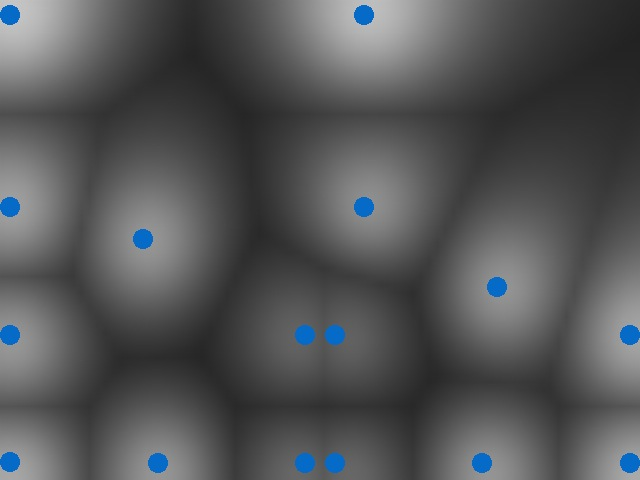
\includegraphics[width=\columnwidth]{../ICMC2009-dbap/all_r_6_b_0_2}}}
	% To use when using latex, dvips and ps2pdf
% 	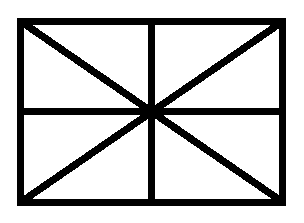
\includegraphics[width=\columnwidth]{figure.eps}}}
%\caption{Figure captions should be placed below the figure}
%\label{fig:example}
%\end{figure}




